\documentclass[useAMS, usenatbib]{mnras}
\pdfsuppresswarningpagegroup=1
%
\usepackage[spanish,es-minimal,english]{babel}
\usepackage[utf8]{inputenc}
\usepackage{graphicx}
\graphicspath{{tere-figs/}{figs/}}

\usepackage{xcolor}
\usepackage{hyperref}
\usepackage{siunitx}
\usepackage{newtxtext}
\usepackage[stix2,smallerops]{newtxmath}
\usepackage{booktabs}
\hypersetup{colorlinks=True, linkcolor=blue!50!black, citecolor=black,
  urlcolor=blue!50!black}
\usepackage{etoolbox}
\robustify\bfseries
\robustify\itshape

\bibliographystyle{mnras}

\sisetup{
  % explicit""+" is useful for velocities
  retain-explicit-plus = true,
  % prefer 10^6 over 1 x 10^6
  retain-unity-mantissa = false,
  % Use x +/- e instead of x(e)  
  separate-uncertainty = true,
  % Make sure to pick up bold font when used in section heading for instance
  detect-weight = true,
}

%%
%% Will macros
%%
% A better \ion command that works in more circumstances
\newcommand\ION[2]{#1\,\scalebox{0.9}[0.8]{\uppercase{#2}}}
\newcounter{ionstage}
\renewcommand{\ion}[2]{\setcounter{ionstage}{#2}% 
  \ensuremath{\mathrm{#1\,\scriptstyle\Roman{ionstage}}}}
\newcommand\hii{\ion{H}{2}}
\newcommand\nii{[\ion{N}{2}]}
\newcommand\oiii{[\ion{O}{3}]}


%%
%% Teresa macros
%%
\newcommand{\Sub}[1]{_\mathrm{#1}}
\newcommand{\SSub}[1]{_\mathrm{\scriptscriptstyle #1}}
\newcommand{\Sup}[1]{^\mathrm{#1}}
\newcommand{\kms}{\ensuremath{\mathrm{km\ s}^{-1}}}
\newcommand{\pcc}{\ensuremath{\mathrm{cm}^{-3}}}
\newcommand{\sii}{[\ion{S}{2}]}
\newcommand{\heii}{\ion{He}{2}}
\newcommand\OIlam{[\ion{O}{1}]\,6300\,\AA\@}
\newcommand\SIIlam{[\ion{S}{2}]\,6731\,\AA\@}
\newcommand\SIIlamshort{[\ion{S}{2}]\,6716\,\AA\@}
\newcommand\SIIlamboth{[\ion{S}{2}]\,6716,6731\,\AA\@}
\newcommand\SIIIlam{[\ion{S}{3}]\,6312\,\AA\@}
\newcommand\NIIlam{[\ion{N}{2}]\,6584\,}
\newcommand\NIIlamlam{[\ion{N}{2}]\,6548,6584\,\AA\@}
\newcommand\OIIIlam{[\ion{O}{3}]\,5007\,\AA\@}
\newcommand\HeIIlam{HeII\,4686\,\AA\@}
\newcommand\Halam{H$\alpha$\,6563\,\AA\@}
\newcommand\Ha{\ensuremath{\mathrm{H}\alpha}}
\newcommand\Hb{\ensuremath{\mathrm{H}\beta}}
\newcommand{\vhel}{\ensuremath{V_\mathrm{hel}}}
\newcommand{\vmean}{\ensuremath{\langle V\rangle}}
\newcommand{\vsys}{\ensuremath{V_\mathrm{sys}}}
\newcommand{\vexp}{\ensuremath{V_\mathrm{exp}}}
\newcommand{\hr}{\ensuremath{^\mathrm{h}}}
\newcommand{\minute}{\ensuremath{^\mathrm{m}}}
\newcommand{\teff}{\ensuremath{T_\mathrm{eff}}}


\title{The complex structure and peculiar internal motions of the planetary nebula NGC 6210}

%\author{Ma.\ T. Garc\'{\i}a-D\'{\i}az, J. A. L\'opez, W. Steffen \& 
%  M. G., Richer 
% \affil{Instituto de Astronom\'ia,
%    Universidad Nacional Aut\'onoma de M\'exico} Campus Ensenada,
%  Ensenada, Baja California, 22800, M\'exico}
%\affil{tere@astrosen.unam.mx, jal@astrosen.unam.mx, wsteffen@astrosen.unam.mx, richer@astrosen.unam.mx}

\author[López et al.]{
  J. A. López,\(^1\)\thanks{
    jal@astro.unam.mx,
    tere@astro.unam.mx,
    w.henney@irya.unam.mx,
    richer@astro.unam.mx
  }
  Ma.\ T. García-Díaz,\(^1\)\footnotemark[1]
  William J. Henney\(^2\)\footnotemark[1]
  and M. G. Richer\(^1\)\footnotemark[1]
  \\
  \(^1\)\foreignlanguage{spanish}{
    Instituto de Astronomía,
    Universidad Nacional Autónoma de México,
    Ensenada, Baja California, 22800, México}
  \\
  \(^2\)\foreignlanguage{spanish}{
    Instituto de Radioastronomía y
    Astrofísica, Universidad Nacional Autónoma de México, Apartado
    Postal 3-72, 58090 Morelia, Michaoacán, Mexico}
}
% These dates will be filled out by the publisher
\date{Accepted XXX. Received YYY; in original form ZZZ}

% Enter the current year, for the copyright statements etc.
\pubyear{2020}




\begin{document} 
\label{firstpage}
\pagerange{\pageref{firstpage}--\pageref{lastpage}}
\maketitle

\begin{abstract}
  A comprehensive kinematic study has been carried out on the planetary nebula (PN) NGC 6210. Multiple long-slits, echelle spectra have been obtained over the face of this nebula mapping its full shell structure, the opposite pairs of extended, twisted arms and the bipolar collimated outflows and bullets. Public {\it HST} imagery has been used to identify kinematic elements with structural components. The long-slit spectroscopic information has been combined into channel maps that greatly facilitate visualizing the otherwise intricate expansion pattern of this  planetary nebula. The global morphology of NGC 6210 is  reminiscent of other planetary nebulae with extended X-ray emission, suggesting the presence of a central hot bubble produced by shocked stellar wind. In spite of the dramatic structure of this PN substantial expanding radial motions are only found in the material surrounding the central, inner shell. The slow radial motions of the collimated outflows and the bullet-like knots indicate that they are  moving away from the core very close to the plane of the sky, nearly perpendicular to the line of sight
\end{abstract}


\begin{keywords}
  Planetary Nebulae: individual (NGC~6210)
  -- ISM: kinematics and dynamics -- ISM blowout
  -- techniques: imaging spectroscopy
\end{keywords}

\maketitle

\section{INTRODUCTION}
\label{sec:introduction}
NGC 6210 is a bright and relatively large PN in the northern sky. The first photographic image of NGC 6210 was published by \citet{Duncan37}. In that old, fuzzy image a pair of twisted arms protruding in opposite directions from a blurred,  bright, nebular core are apparent. Several studies have discussed the inner kinematic motions of this object, e.g. \citet{Osterbrock66, Weedman68, Becker84, Icke89}. However, none of those studies had the spatial coverage and spectral resolution needed to produce a reliable spatio-kinematic model of this PN. 
The best kinematic study to date on NGC 6210 is probably the one published by \citet{Phillips96}  who obtained 11 long-slits centered on the nebular core, with each slit at different position angles thus providing a good spatial coverage but with only limited, low and medium spectral resolution. From these data  they suggested a  reasonable kinematic model for the ionized nebula. NGC 6210 jumped into fame thanks to the {\it HST} images obtained during the 1996 - 1998 period under the observing programs 6347 (K. Borkowski), 6792 (R. Rubin), 7501 (A. Hajian)  and 11122 (B. Balick). These images showed for the first time the extraordinarily complex morphology of NGC 6210. Incidentally the  {\it HST} and ground-based imagery prompted the nickname "the turttle" for this nebula, given the shape of its main body and extended arms that resemble the shell of a turttle with a long neck and its fins. The distance estimates to NGC 6210 vary roughly from 1.5 to 2.0 kpc. \citep{Hajian95} derive a distance to NGC 6210 from VLA 6 cm  expansion parallax measurements of 1.57$\pm0.40$ kpc, considering an expansion distance of 23 \kms 

In this work we present a thorough spectral mapping of all the morphological elements of the PN obtained at high spectral resolution that allow 
disentangling the various spatio-kinematic components and provide and overall view of its structure and evolution. Radial velocities are combined with 2-epoch HST \oiii and \nii archive image sets (http://archive.stsci.edu/) to derive proper motions. Individual long-slit echelle data obtained over N observing runs are combined into emission and velocity channel maps that serve as an excellent tool to visualize and understand the peculiar velocity fields, of the several structural components.

In Section 2, we describe our observations and the data-reduction steps, In Section 3 we describe the velocity-channel map of emission. In Section 4, we discuss the radial velocities and proper motions of the nebula. In Seccion 5 we present the discussion and conclusion.

\section{OBSERVATIONS AND DATA REDUCTION}
\label{sec:observations}

Long-slit, echelle, spectroscopic observations of the nebula NGC~6210
were performed with the 2.1~m telescope at the Observatorio
Astron\'omico Nacional at San Pedro M\'artir, (OAN-SPM), Baja
California, M\'exico. We used the Manchester Echelle Spectrometer
(MES-SPM) \citep{Meaburn03} on the 2.1 m telescope in its $f$/7.5
configuration.  The MES-SPM is a long-slit, echelle spectrometer that
has no cross-disperser; it isolates single orders using interference
filters. For the 2003, 2004 and 2011 of the present observations, we used a
SITE-3 CCD detector with 1024 $\times$ 1024 square pixels, each 24
$\mu$m on a side ($\equiv$0.312 arcsec pixel$^{-1}$). The detector
was set to a binning of 2 $\times$ 2 in both the spatial and spectral
directions. Consequently, 512 increments, each 0\farcs624{} long gave
a projected slit length of 5\farcm32 on the sky. A TEK-1 CCD detector
was used for the 1998 data set with 1024$\times$1024 pixels$^2$ with
sides measuring 24 $\mu$m, using 2$\times$2 binning ($\equiv$0.62 arcsec
pixel$^{-1}$ and 3.5 \kms pixel$^{-1}$). For the 2001 and 2013 we used
a Marconi CCD detector with 2048 $\times$ 2048 square pixels, each 13.6
$\mu$m on a side. The detector was set to a binning of 2 $\times$ 2 in
both the spatial and spectra directions. Consequently, 1024
increments, each 0\farcs352{} long gave a projected slit length of
5\farcm47 on the sky.

We used a 90\,\AA\, and 50\,\AA\, bandwidth
filter to isolate the 87th and 114th orders containing the
\Ha\,$+$\,\NIIlam\, and \OIIIlam\, nebular emission lines,
respectively. We used a 70~$\mu$m{} ($\equiv$0.95\arcsec) slit, giving
a velocity resolution of 9.2 \kms{} ($\equiv$0.312 arcsec
pixel$^{-1}$ and 150 $\mu$m{} ($\equiv$1\farcs 9 and $\equiv$11.5
\kms) slit.


We obtained 23 consecutive and tightly spaced positions over the
NGC~6210. The slit positions are indicated and labeled in Figure~1 on
a WFPC~2 image of the NGC~6210 obtained from the HST archive. In order
to establish the exact position of the slit in each pointing, the slit
position on the sky was recorded with an automatic procedure available
in MES-SPM prior to the spectroscopic exposure.

The log of spectroscopy observation is given in Table 1 divided into
dates, number of spectra, exposure times, spectral range, resolution,
slit wide, position angle and name of the slit (see Figure~1). 
The high resolution data are available in San Pedro M\'artir Kinematic Catalogue
of Galactic Planetary Nebulae (http://kincatpn.astrosen.unam.mx)
\citep{Lopez12}.


Due to saturation of several slit positions on the nebula, we obtained a 
new set of observation on August 13, 2015. We used the same detector as 
that used for the 2015 dataset, which was a E2V-4240 (Marconi 2)  detector 
with 2048$\times$2048 pixels$^2$ 
with sides measuring 13.5 $\mu$m, using 2$\times$2 binning 
($\equiv$0.531 arcsec pixel$^{-1}$. Spectra were obtained at 11 different 
positions across the nebula, with exposure times of 1800 seconds. The slit 
was oriented N-S. 

An additional slit was placed outside the nebula 
to detect The outer halo of NGC 6210. The observation was carried out on 18 September 2019.  The spectrum was obtained in order 87 (H alpha and [N II] lines) with the 150 micron slit oriented at position angle of 56 degrees.  The detector was an E2V 2048x2048 CCD with 13.5 $\mu$/pix used in binning 3$\times$3.  The spectral dispersion was 0.084 \AA/pix and the plate scale 0.175\arcsec/pixel.

The characteristics of the observations are listed in Table 2.

\begin{table*}
\centering
\caption{Log  of Time-resolved  Observations of {\bf NGC~6210}.}
\begin{tabular}{l|ccccccc} \hline 
&  \multicolumn{7}{c}{Spectroscopy hight resolution/ 2.1m  OAN-SPM}            \\[0.1pt]
\hline 
Run    &   Exp. Time & Range  & slit & P. A.   & slit        \\
DD/MM/YYYY   &     frame         &    (s)   &  (\AA)    &    (\AA)  & (m$\mu$) & (degree) & name    \\[1pt]   \hline 
28/06/1998          & 30 & H$\alpha$  & 150 & 90 & o\\
28/06/1998          & 300 & H$\alpha$  & 150 & 90 & n\\
28/06/1998           & 1200 & H$\alpha$   & 150 & 90 & m,p,q \\
05/06/2003         & 1800 &  H$\alpha$   & 70 &0 & f,e,d,h,i,k,b\\ 
16/10/2003   &  1800 &   H$\alpha$    & 70 & $-$21 & t\\
16/10/2003    &  1800 &   H$\alpha$   & 70 & $-$68 & v\\
17/10/2003    &  1800 &   H$\alpha$  & 70 & 77 & w\\
13/06/2004   & 1800 &   O\sc{iii}  & 70 & $-$9 & r  \\  
13/06/2004   & 1800 &   O\sc{iii}  & 70 & $-$19 & s  \\  
14/06/2004    & 1800 &   S\sc{ii} &150 & $-$19 & s  \\
13/06/2004   & 1800 &   O\sc{iii}  & 70 & $-$56 & u  \\  
14/06/2004   & 1800 &   O\sc{iii}  & 150 & 0 & a,l  \\
21/05/2011     & 1800 & H$\alpha$  & 150 & 0 & g \\
21/05/2011     & 600 & O\sc{iii} & 150 & 0  & g\\
06/07/2013    &  1800 & H$\alpha$   & 150 & 0 & c,i,j \\
20/08/2005   & 3 &  1800 &   H$\alpha$, [OIII]    & 0.26 & 70 & 0 & h, j, k\\
\hline
\hline 
\end{tabular}
\label{table:pa5}
\end{table*}


\begin{table*}
\centering
\caption{Log  of Time-resolved  Observations of {\bf NGC~6210}. Epoch 2015}
\begin{tabular}{l|ccccccc} \hline 
&  \multicolumn{7}{c}{Spectroscopy hight resolution/ 2.1m  OAN-SPM}            \\[0.1pt]
\hline 
Run   &   Exp. Time & Range  & slit & P. A.   & slit        \\
DD/MM/YYYY   &     frame         &    (s)   &  (\AA)    &    (\AA)  & (m$\mu$) & (degree) & name    \\[1pt]   \hline 
18/08/2015  &  1800 &   H$\alpha$, [OIII]  & 70 & 0 & c, d, e, f, g\\
19/08/2015  &  1800 &   H$\alpha$, [OIII]   & 70 & 0 & b, a, i\\
19/08/2015  &  1800 &   H$\alpha$    & 70 & 0 & b, a, i\\
18/09/2019  &  1800 &   H$\alpha$    & 150 & 56 & \\

\hline
\hline 
\end{tabular}
\label{table:pa5}
\end{table*}

All data was reduced (bias removal 
and cosmic-ray removal) by using standard IRAF\footnote{IRAF is
  distributed by the National Optical Astronomy Observatory, which is
  operated by the Association of Universities for Research in
  Astronomy, Inc. under cooperative agreement with the National
  Science foundation}.
  This was followed by rectification and first-order wavelength 
  calibration of the two-dimensional spectra based on the comparison
  the spectrum
of a Th/Ar lamp to an accuracy of $\pm$1 \kms{} when converted to
radial velocity.  All spectra presented in this paper are corrected to
heliocentric velocity (\vhel). 
The Figure 3 shows the position-velocity ({\it P-V})  arrays of \Halam\,
\NIIlam \AA, \OIIIlam, respectively, where the heliocentric velocities are used,
and positions are specified as arcsecond offsets (x,y).

Using FORTRAN and phython routines, we produced  velocity cubes in  \NIIlam{} and \oiii{} emission lines, in order to 
...

The resulting data cubes for the \Halam\, and \NIIlam\, lines are shown
in Figure 3 as isovelocity channel maps, each isovelocity map is 20
\kms\, wide. 


\section{KINEMATICS}
\label{sec:kinematic}

The Figure 3 shows the \Halam{},  \OIIIlam{}, and \NIIlam{} velocity arrays, {\it P--V}, for all individual slit position, observed on 2015 epoch: \Ha{} {\it P--V} is shown on the left panel,  on
the middle panel is the corresponding \OIIIlam\, {\it P--V} and \NIIlam{} on the right panel. Spatial
offsets are in arcseconds.  The stellar continuum from the central star
has not been subtracted. We derive a heliocentric
systemic velocity, \vsys $=40$~\kms{} by using the slits position f (epoch 2003) and  which passes through the central star. The expansion velocity of the inner shell, v$_{exp}$ = 28 \kms.
\section{PROPER MOTIONS}
 \subsection{Hubble Space Telescope Data} 
The data used in this study to measure the proper motions of the turttle nebula consist of images which were retrieved from the HST archive. The \nii{} observations were made in two separate observing runs: on 1998 June 30, as part of program 7501, with Hajian, Arsen R., as PI. During this run, six images were obtained with the WFPC2, with an exposure time of 100 s (three images) y 40 s (three images) using the F658N filter. The second-epoch data were obtained on 2008 January 18, from the science program 11122, with Bruce Balick, as PI, who employed the same configuration as in program 7501 to acquire three images with the F658N filter, using 400 s exposure times for all of them. For all of the images, we used the drizzled images (processed with Astrodrizzle). 


\vfill \eject

%\bibliographystyle{astroads}
\begin{thebibliography}{}


\bibitem[L\'opez et al.(2012)]{Lopez12} L\'opez, J. A., Richer, M. G.,
  Garc\'ia-D\'iaz, M. T., Clark, D. M., Meaburn, J., Riesgo, H., Steffen,
  W., \& Lloyd, M. 2012, RevMexAA, 48, 3

\bibitem[Meaburn et al.(2003)]{Meaburn03} Meaburn, J., L\'opez,
J. A., Guti\'errez, L., Quir\'oz, F., Murillo, J. M. \& Vald\'ez, J.
2003, RMxAA, 39, 185M

\bibitem[Osterbrock et al.(1966)]{Osterbrock66} Osterbrock, D. E., Miller,
  J. S., \& Weedman, D. W. 1966, \apj, 145, 697

\bibitem[Weedman(1968)]{Weedman68} Weedman, D. W. 1968, \apj, 153, 49

\bibitem[Becker et al.(1984)]{Becker84} Becker, I., Gieseking, F. \& Solf, J.1984, 
Mitteilungen der Astronomishen Gesellschaft Hamburg, 62, 253

\bibitem[Icke et al.(2005)]{Icke89} Icke, V., Preston, H. \& Balick, B.
 1989, \aj, 97, 4621



\bibitem[Balick et al.(1998)]{Balick98} Balick B., Alexander J.,
  Hajian A. R., Terzian Y., Perinotto M., \& Patriarchi P. 1998,
  \apj, 116, 360

\bibitem[Balick et al.(1987a)]{Balick87a} Balick, B., Preston, H. L.,
  Icke, V. 1987a, \aj, 94, 1641B



\bibitem[Balick(1987c)]{Balick87c} Balick B. 1987c, \aj, 94, 671

\bibitem[Ciardullo et al.(1999)]{Ciardullo99} Ciardullo, R., Bond,
  H. E., Sipior, M. S., Fullton, L. K., Zhang, C.-Y., Schaefer,
  K. G. 1999, \aj, 118, 488
  
 \bibitem[Clark et al.(2010)]{clark10} Clark, D.~M., 
Garc{\'{\i}}a-D{\'{\i}}az, M.~T., L{\'o}pez, J.~A., Steffen, W.~G., 
\& Richer, M.~G.\ 2010, \apj, 722, 1260 

\bibitem[Duncan (1937)]{Duncan37} Duncan, J. C.. 1937, \apj 86, 496
  
\bibitem[Frew(2008)]{Frew08} Frew, D. J. 2008, Ph.D. Thesis, Department of Physics,
  Macquire University, NSW, 2109, Australia
  
 \bibitem[Garc{\'{\i}}a-D{\'{\i}}az et al.(2009)]{gd09} 
Garc{\'{\i}}a-D{\'{\i}}az, M.~T., Clark, D.~M., L{\'o}pez, J.~A., Steffen, 
W., \& Richer, M.~G.\ 2009, \apj, 699, 1633 

\bibitem[Garc\'ia-D\'iaz \& Henney(2007)]{Garcia07} Garc\'ia-D\'iaz,
  Ma. T., \& Henney, W. J. 2007, \aj, 133, 952G

\bibitem[Gieseking et al.(1985)]{Gieseking85} Gieseking, F., Becker,
  I., \& Solf, J. 1985, \apj, 295L, 17G
  
\bibitem[Phillips \& Cuesta(1996)]{Phillips96} Phillips, J. P. \& Cuesta, L. 1996
, \aj, 111, 1227

\bibitem[Hajian \& Terzian(1995)]{Hajian95} Hajian, Y. \&  Terzian, Y., 1995, \aj 109 2600





\bibitem[Heap(1977)]{Heap77} Heap, S. R. 1977, \apj, 215, 864

\bibitem[Kastner et al.(2012)]{Kastner12} Kastner et al. 2012, arXiv:1204.6055

\bibitem[Kudritzki et al.(1997)]{Kudritzki97} Kudritzki, R. P., Mendez,
  R. H., Puls, J., McCarthy, J. K. 1997, IAUS, 180, 64

  
\bibitem[L\'opez et al.(2012a)]{lophb5} L\'opez, J. A., Garc\'{\i}a-D\'{\i}az, M. T., Steffen, W., Riesgo, H. \& Richer, M. G. 2012a, \apj, 750, 131


\bibitem[M\'endez et al.(2011)]{Mendez11} M\'endez, R. H., Urbaneja,
  M.A., Kudritzki, R. P. \& Prinja, R. K. 2011, IAUS 283, submitted.


  
\bibitem[O'Dell et al.(2002)]{Odell02} O'Dell, C. R., Balick, B., Hajian, A. R., Henney, W. J.
  \& Burkert, A. 2002, \aj 123, 3329


\bibitem[O'Dell \& Ball(1985)]{Odell85} O'Dell, C. R., \& Ball,
  M. E. 1985, \apj, 289, 526

\bibitem[Pauldrach et al.(2004)]{Pauldrach04} Pauldrach, A. W. A.,
  Hoffmann, T. L., \& Mendez, R. H. 2004, \aap, 419, 1111

\bibitem[Phillips \& Cuesta(1999)]{Phillips99} Phillips, J. P., \&
  Cuesta, L. 1999, \aj, 118, 2929

\bibitem[Pottasch et al.(2008)]{Pottasch08} Pottasch, S. R., Bernard-Salas, J.,
  \& Roelling T. L.  2008, \aap, 481, 393

\bibitem[Reed et al.(1999)]{Reed99} Reed, D. S., Balick, B., Hajian, A. R.,
  Klayton, T. L., Giovanardi, S., Casertano, S., Panagia, N., \&Terzian, Y.
  1999, \aj, 118, 2430
  
\bibitem[Stanghellini \& Shaw(2008)]{Stanghellini08}
  Stanghellini, L. \& Shaw, R. A. 2008, \apj, 689, 194
  
 \bibitem[Steffen et~al.(2010)]{shapeWo10} Steffen, W., Koning, N., Wenger, S., Morisset, C., \& Magnor, M.
 2010, IEEE, Transactions on Visualization and Computer Graphics, 17, No. 4, 454 


 
  
\bibitem[Steffen \& L{\'o}pez(2006)]{shapeWo06} Steffen, W. \& L{\'o}pez, J.~A.
  2006, RMxAA, 42, 99 

\bibitem[Tinkler \& Lamers(2002)]{Tinkler02} Tinkler, C. M., Lamers,
  H. J. G. L. M. 2002, \aap, 384, 987



\bibitem[Zhang et al.(2012)]{Zhang12} Zhang, Y., Fang, X., Chau, W., Hsia, C.-H., Liu, X.-W., Kwon, S., \& Koning, N. 2012, arXiv:1205.3470

\end{thebibliography}



 % \caption{{\it Left:} Location of each slit position is indicated and
 %   labeled on an HST \OIIIlam, image of the NGC~6210. North is up,
 %   east left}

\begin{figure*}
\centering
  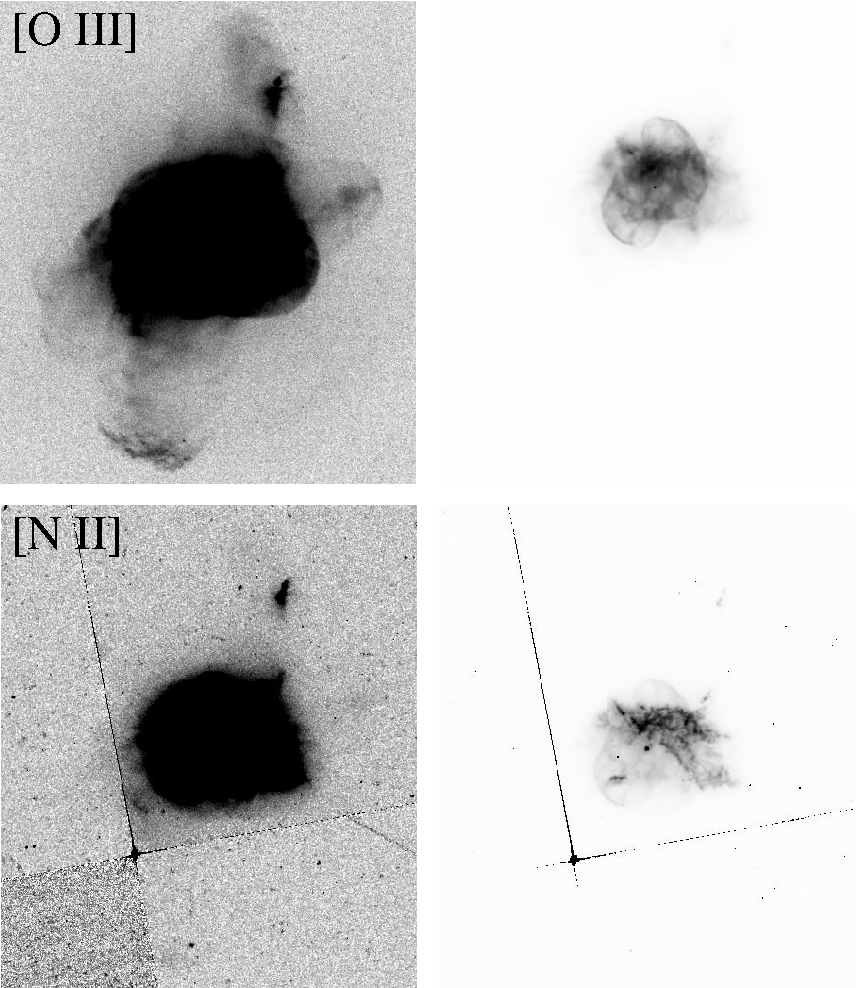
\includegraphics[width=0.7\textwidth]{Figure1.pdf}
  \caption{ }
\end{figure*}

\begin{figure*}
\centering
  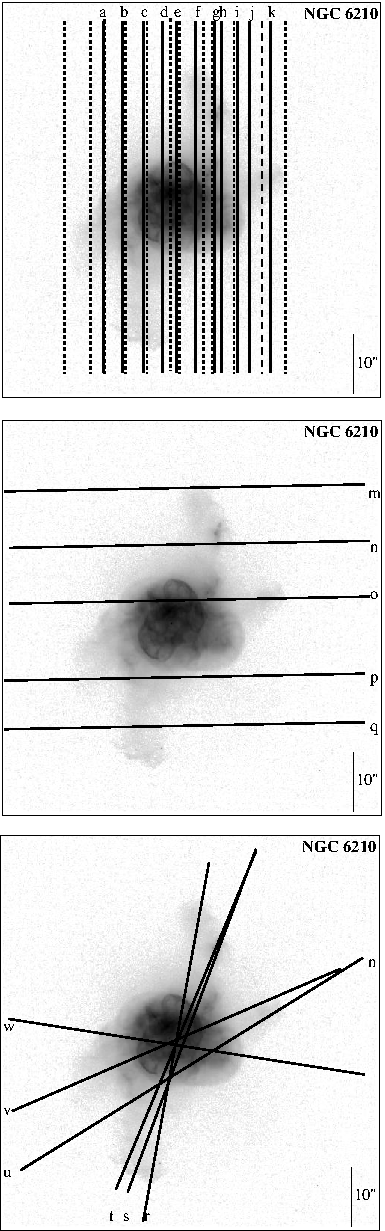
\includegraphics[width=0.4\textwidth]{Figure2a.pdf}
  \caption{ }
\end{figure*}


\begin{figure*}
\centering
  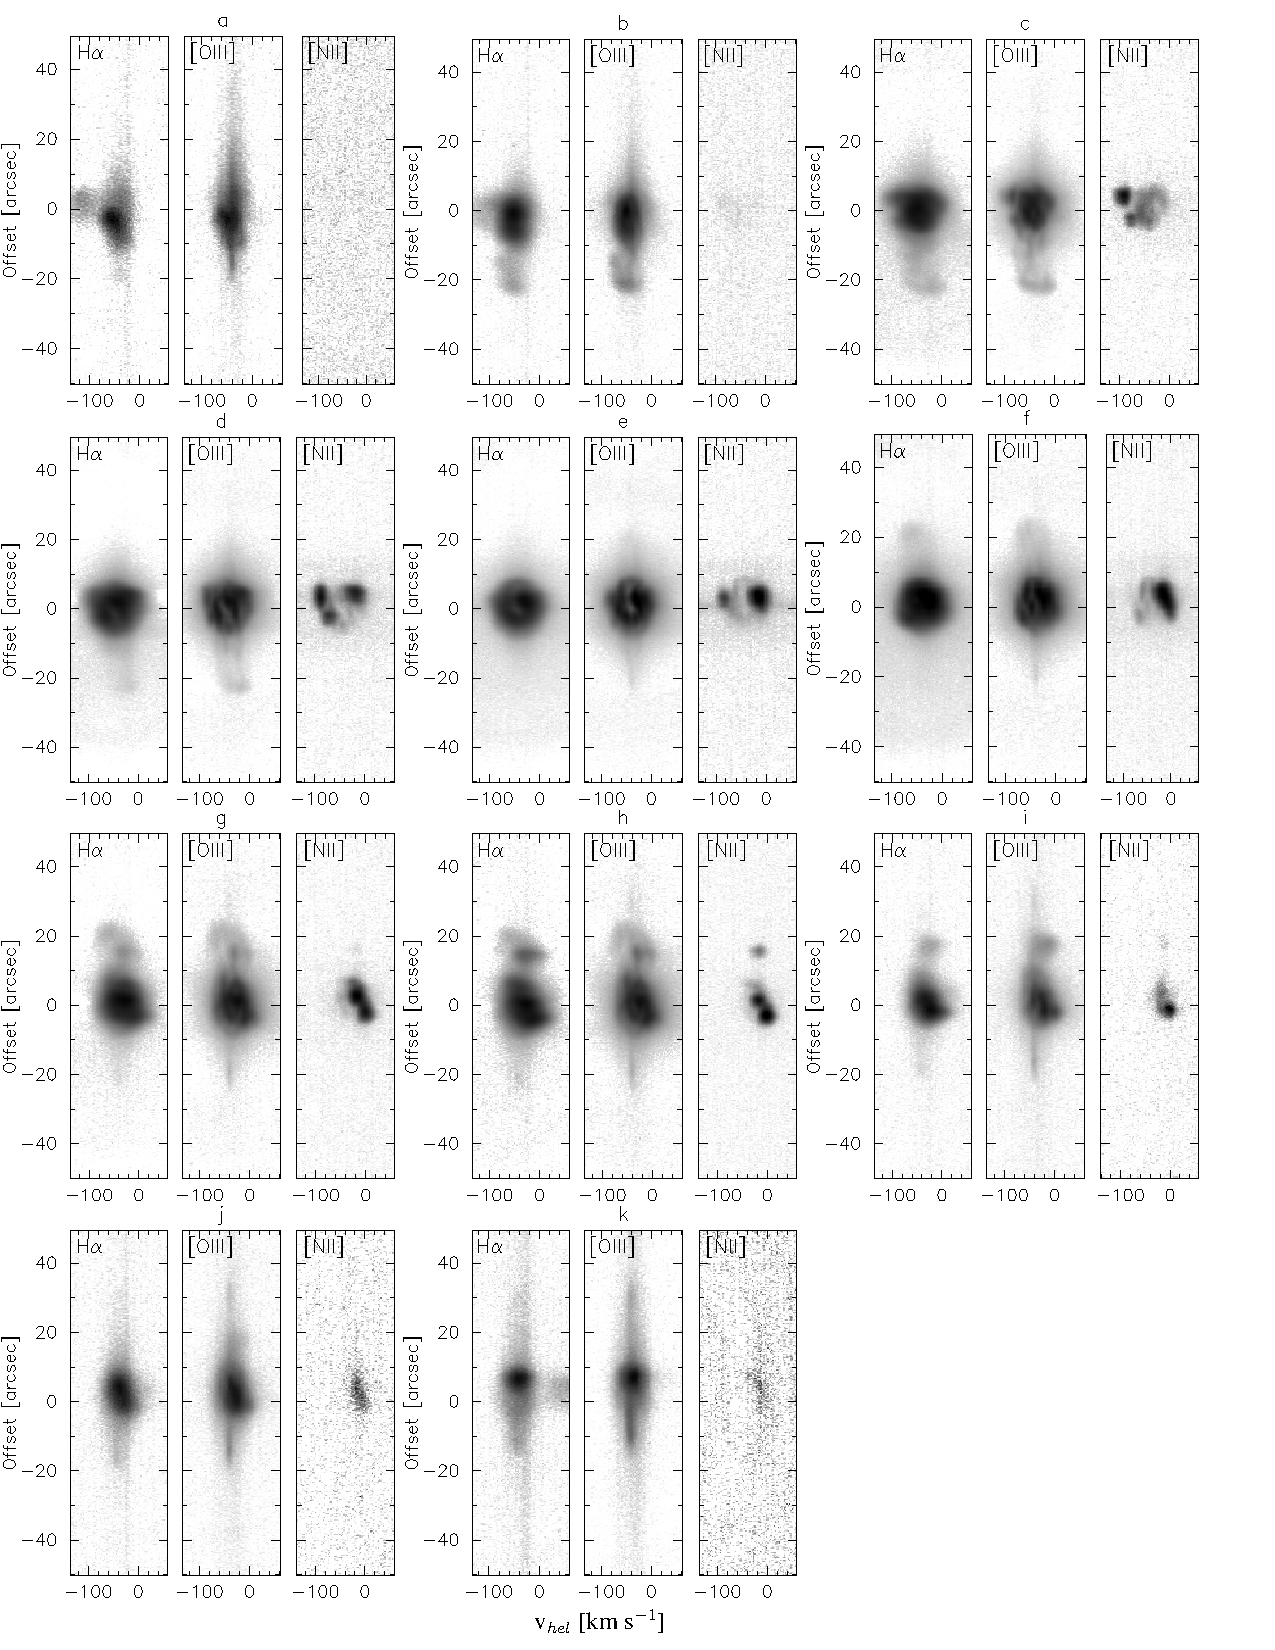
\includegraphics[width=1\textwidth]{Figure3.pdf}
  \caption{ }
\end{figure*}









\begin{figure*}
\centering
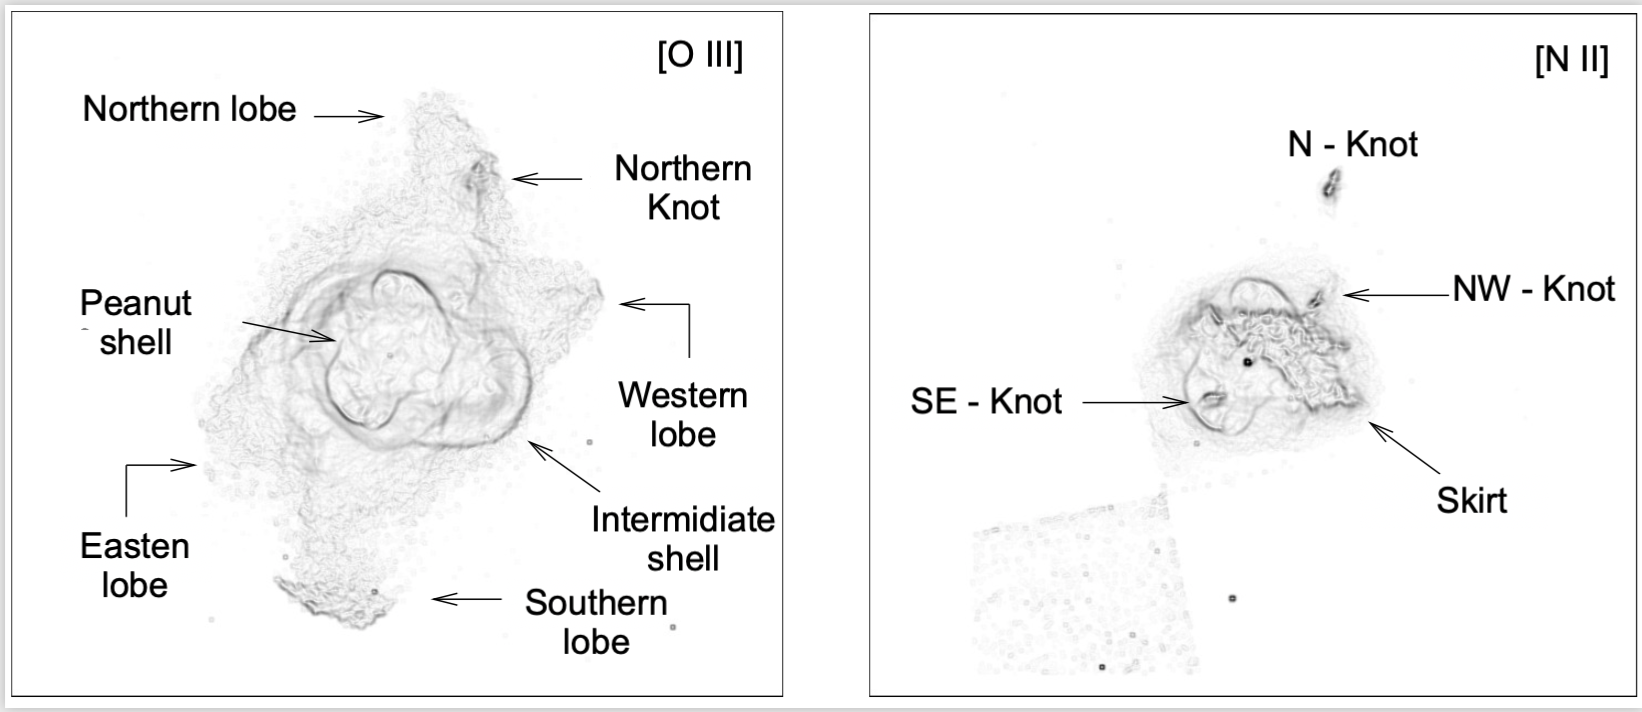
\includegraphics[width=0.9\textwidth]{Figure8.png}
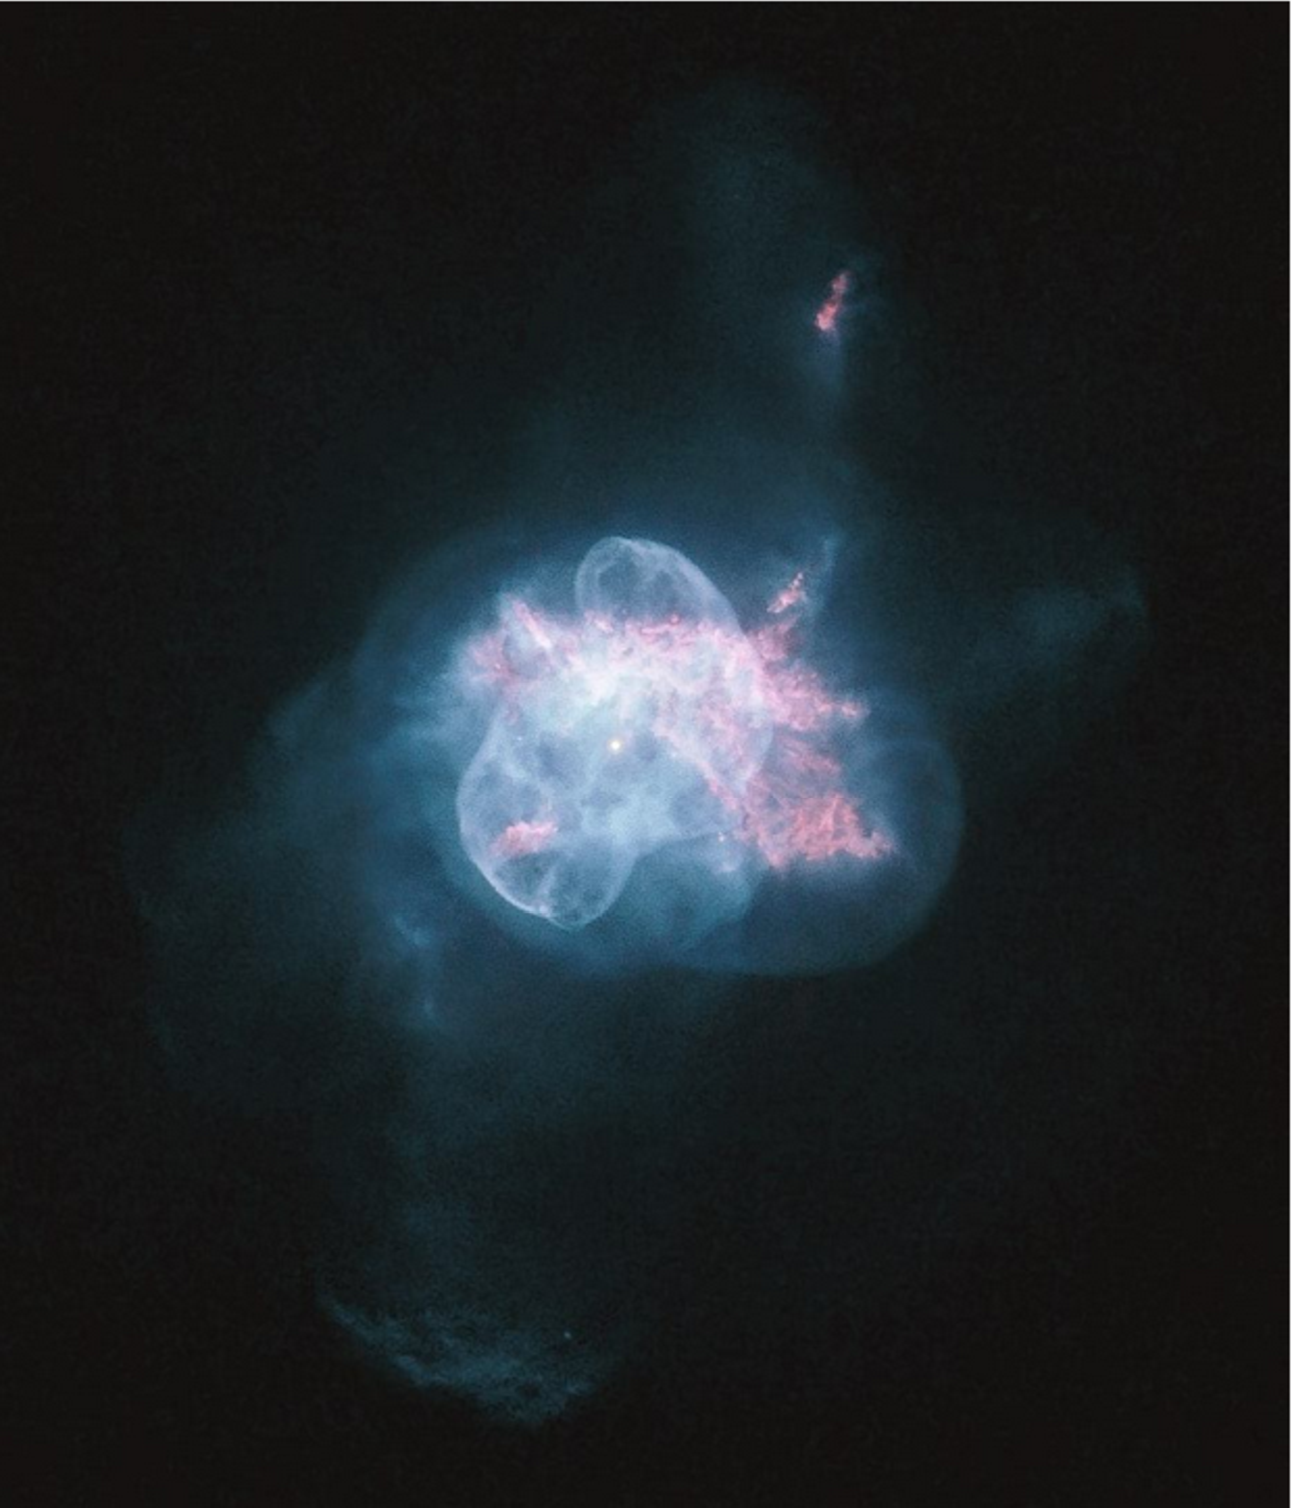
\includegraphics[width=0.42\textwidth]{N6210_ruso.pdf}
\quad
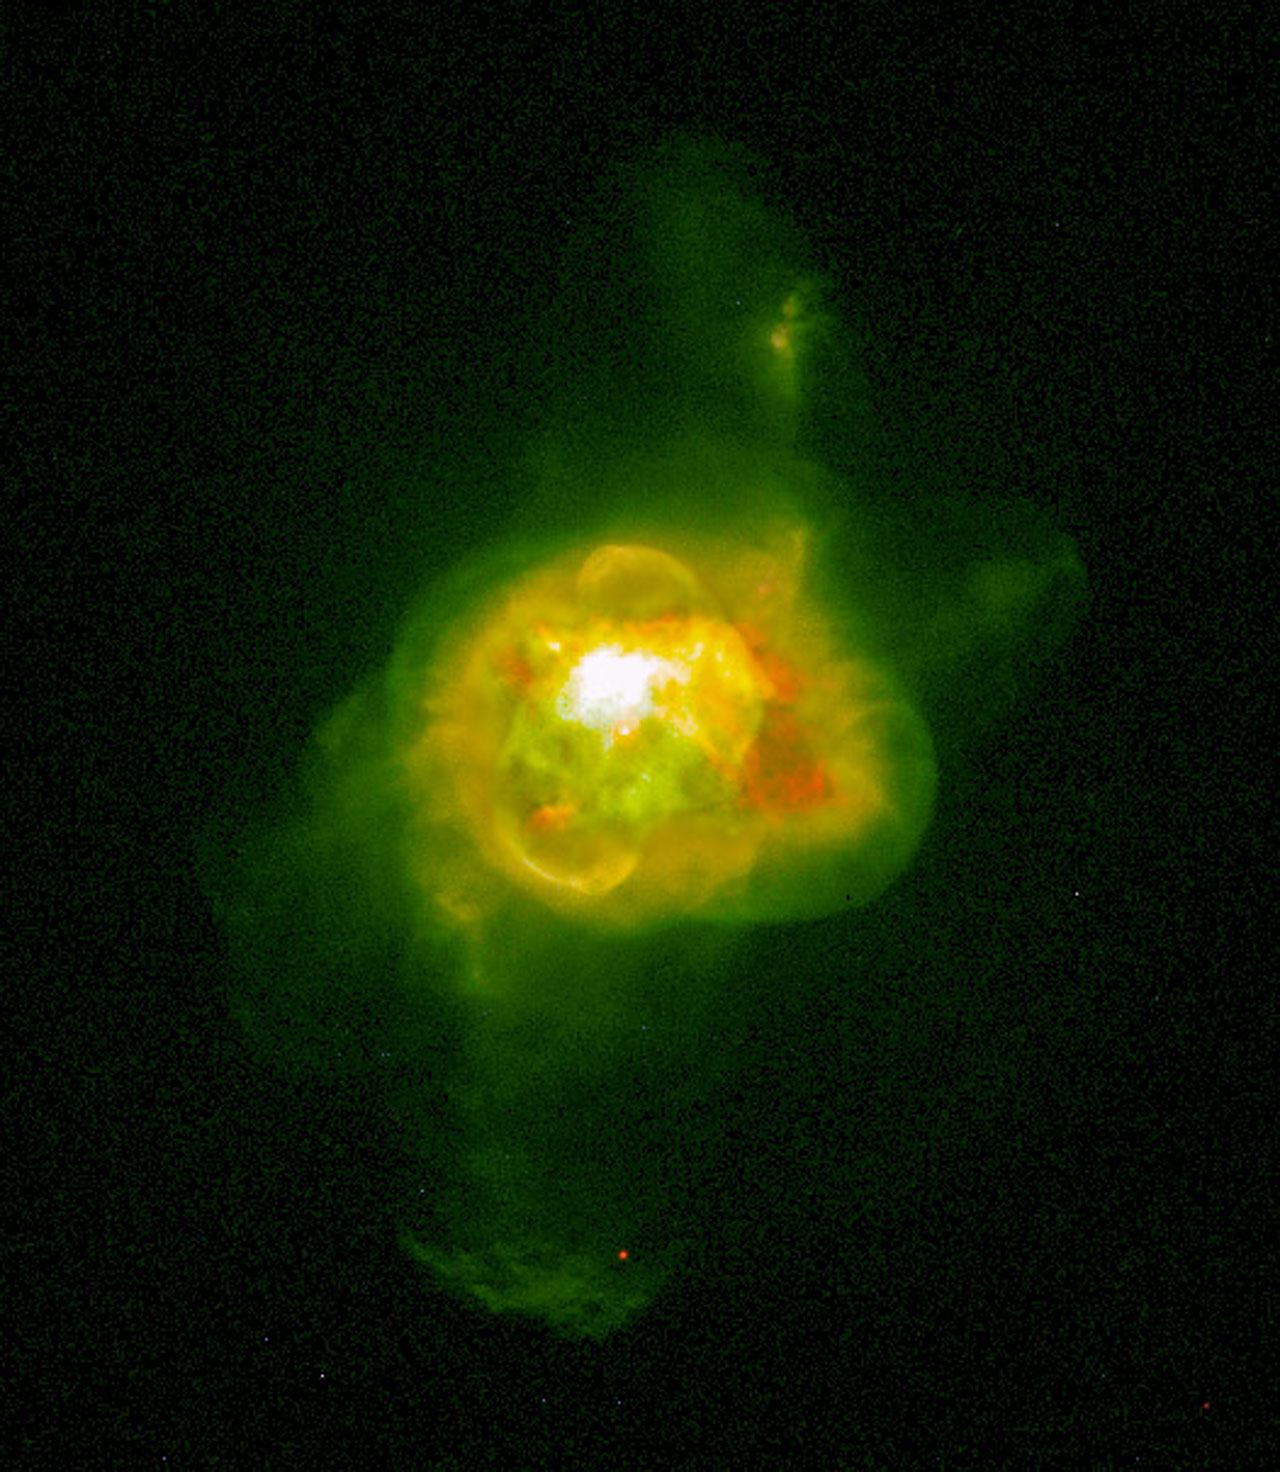
\includegraphics[width=0.427\textwidth]{opo9836f.jpg}
  \caption{}
\end{figure*}





\begin{figure*}
\centering
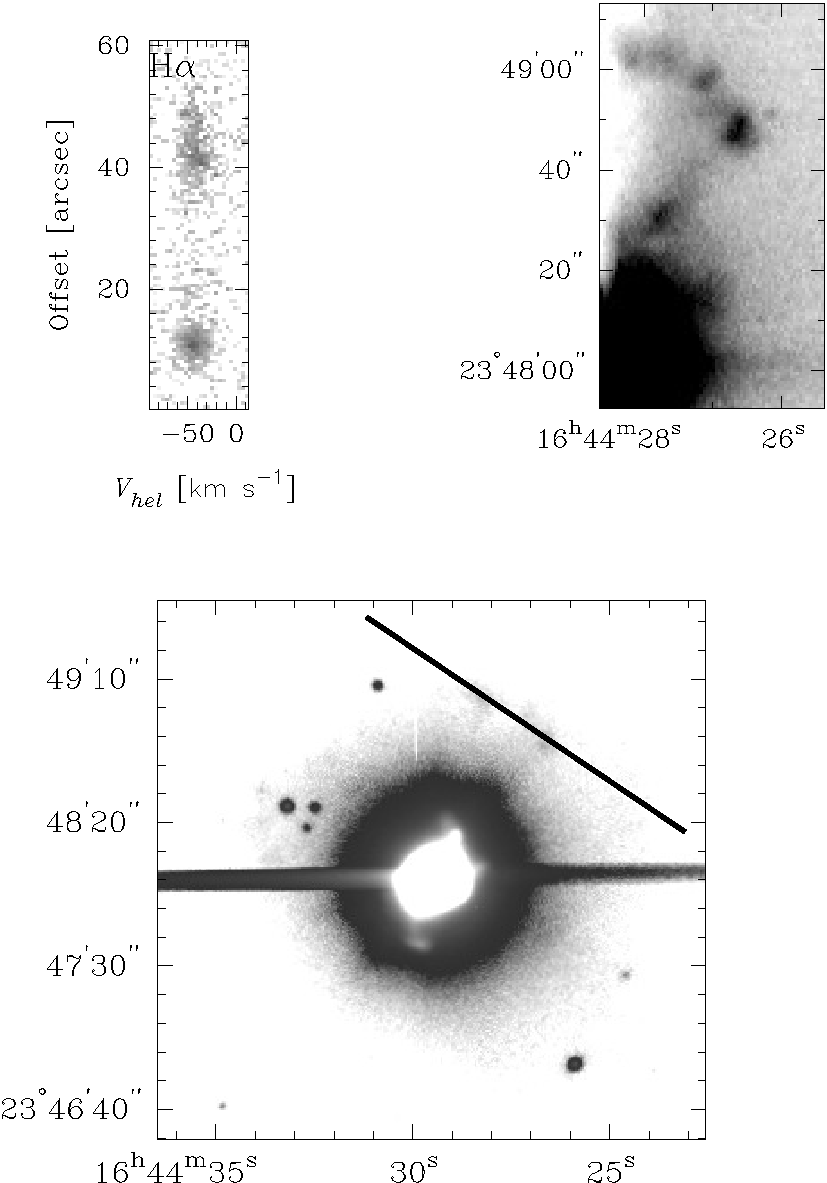
\includegraphics[width=0.9\textwidth]{Figure6.pdf}
  \caption{  }
\end{figure*}





\begin{figure*}
\centering
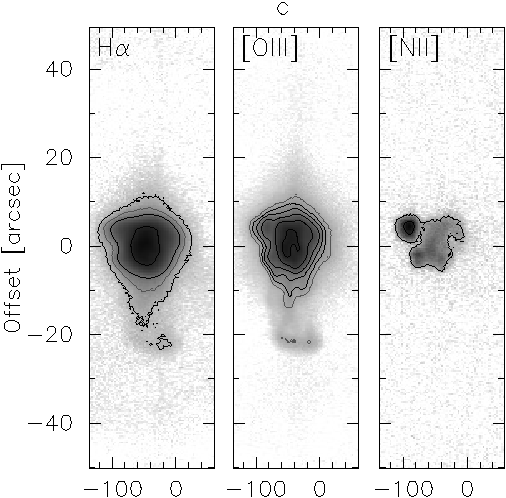
\includegraphics[width=0.9\textwidth]{rendija-c-cont.pdf}
  \caption{  }
\end{figure*}



\begin{figure*}
\centering

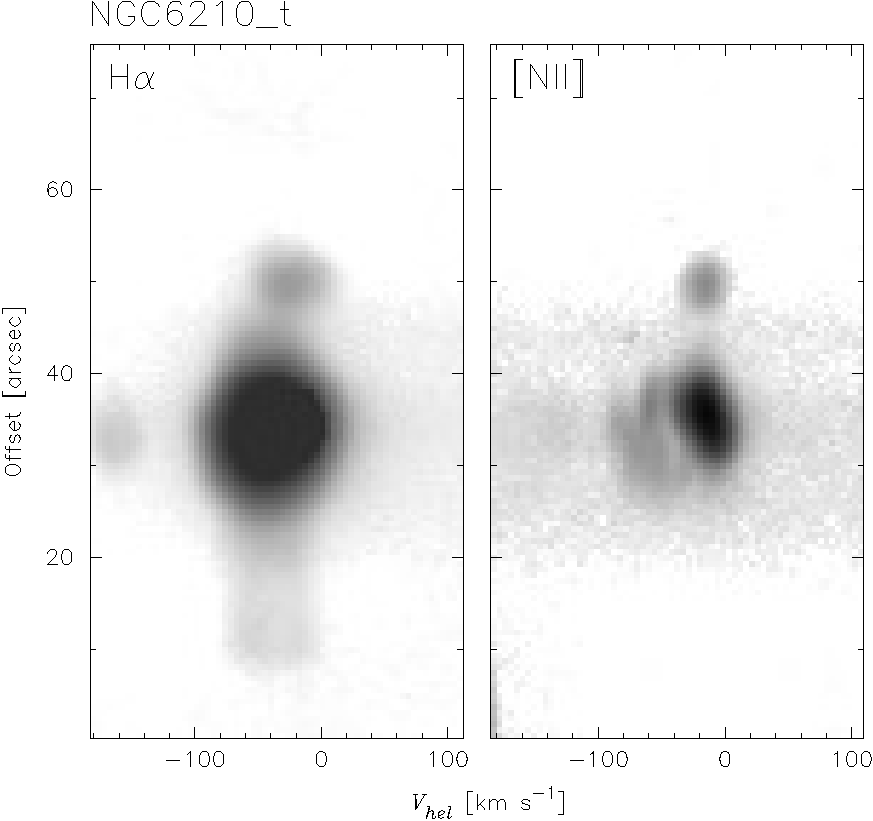
\includegraphics[width=0.4\textwidth]{slit_t_ha_nii.pdf}
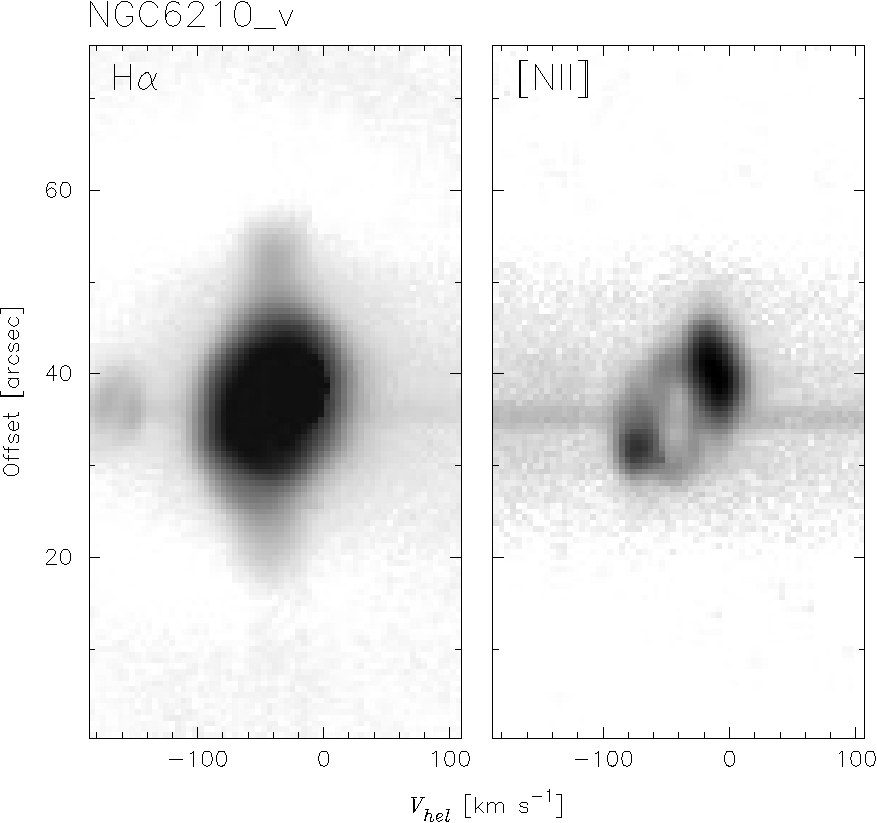
\includegraphics[width=0.4\textwidth]{slit_v_ha_nii.pdf}
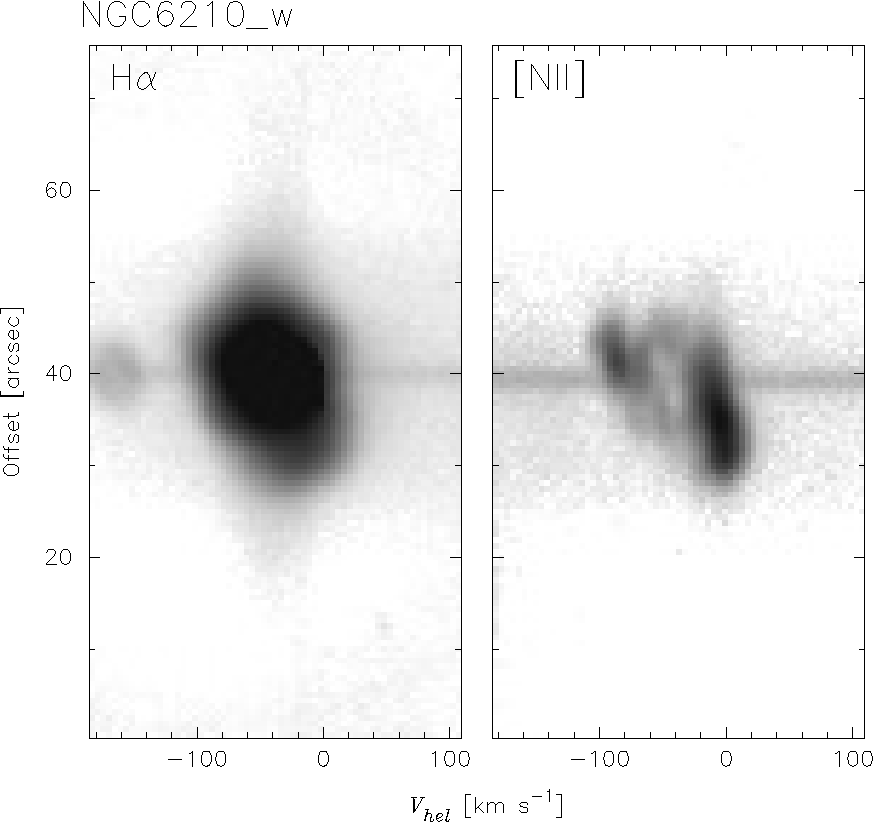
\includegraphics[width=0.4\textwidth]{slit_w_ha_nii.pdf}
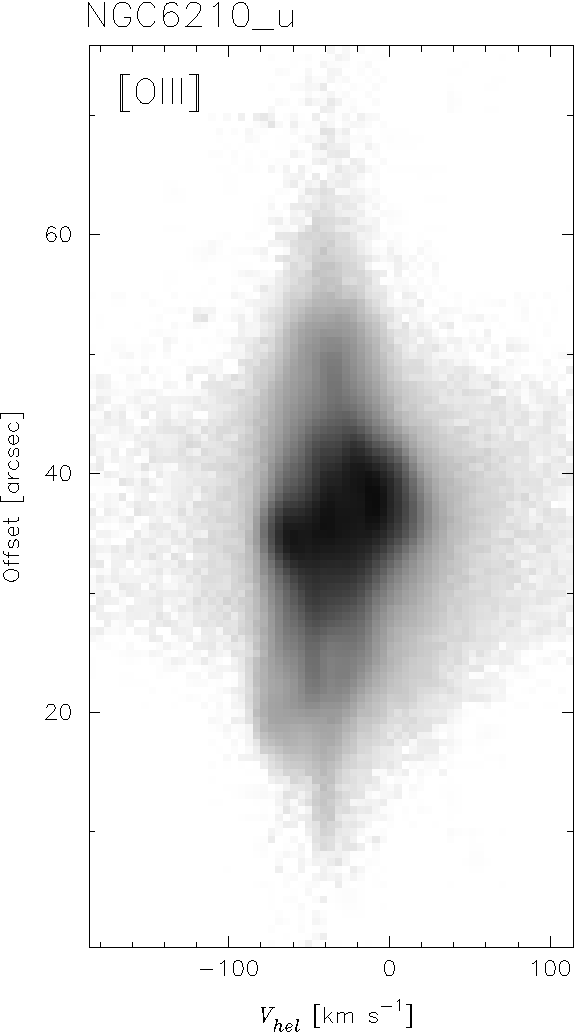
\includegraphics[width=0.2\textwidth]{slit_u_oiii.pdf}
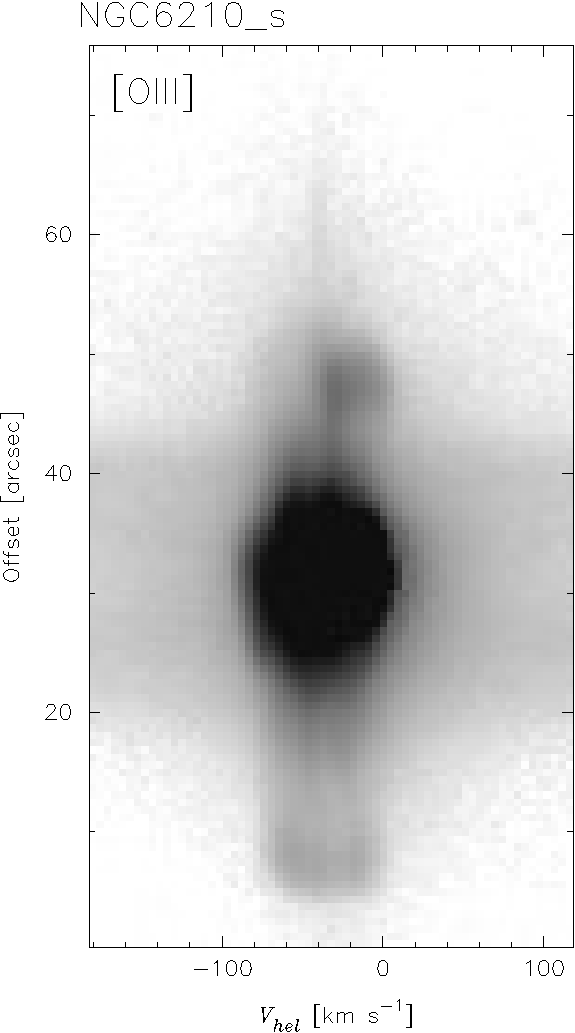
\includegraphics[width=0.2\textwidth]{slit_s_oiii.pdf}
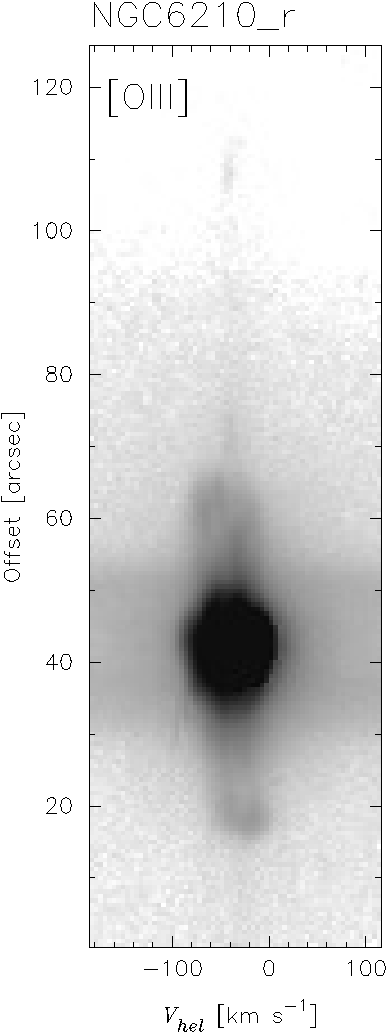
\includegraphics[width=0.2\textwidth]{slit_r_oiii.pdf}

  \caption{  }
\end{figure*}




% Don't change these lines
\bsp	% typesetting comment
\label{lastpage}

\end{document}
%%% Local Variables:
%%% mode: latex
%%% TeX-master: t
%%% End:
